% ============================================================
%  Rozdział 6 — Bezpieczeństwo
% ============================================================
\section{Bezpieczeństwo}

% ------------------------------------------------------------
\subsection{Znaki wodne}
% ------------------------------------------------------------

\begin{figure}[H]
  \centering
  \begin{subfigure}[t]{0.48\linewidth}
    \centering
    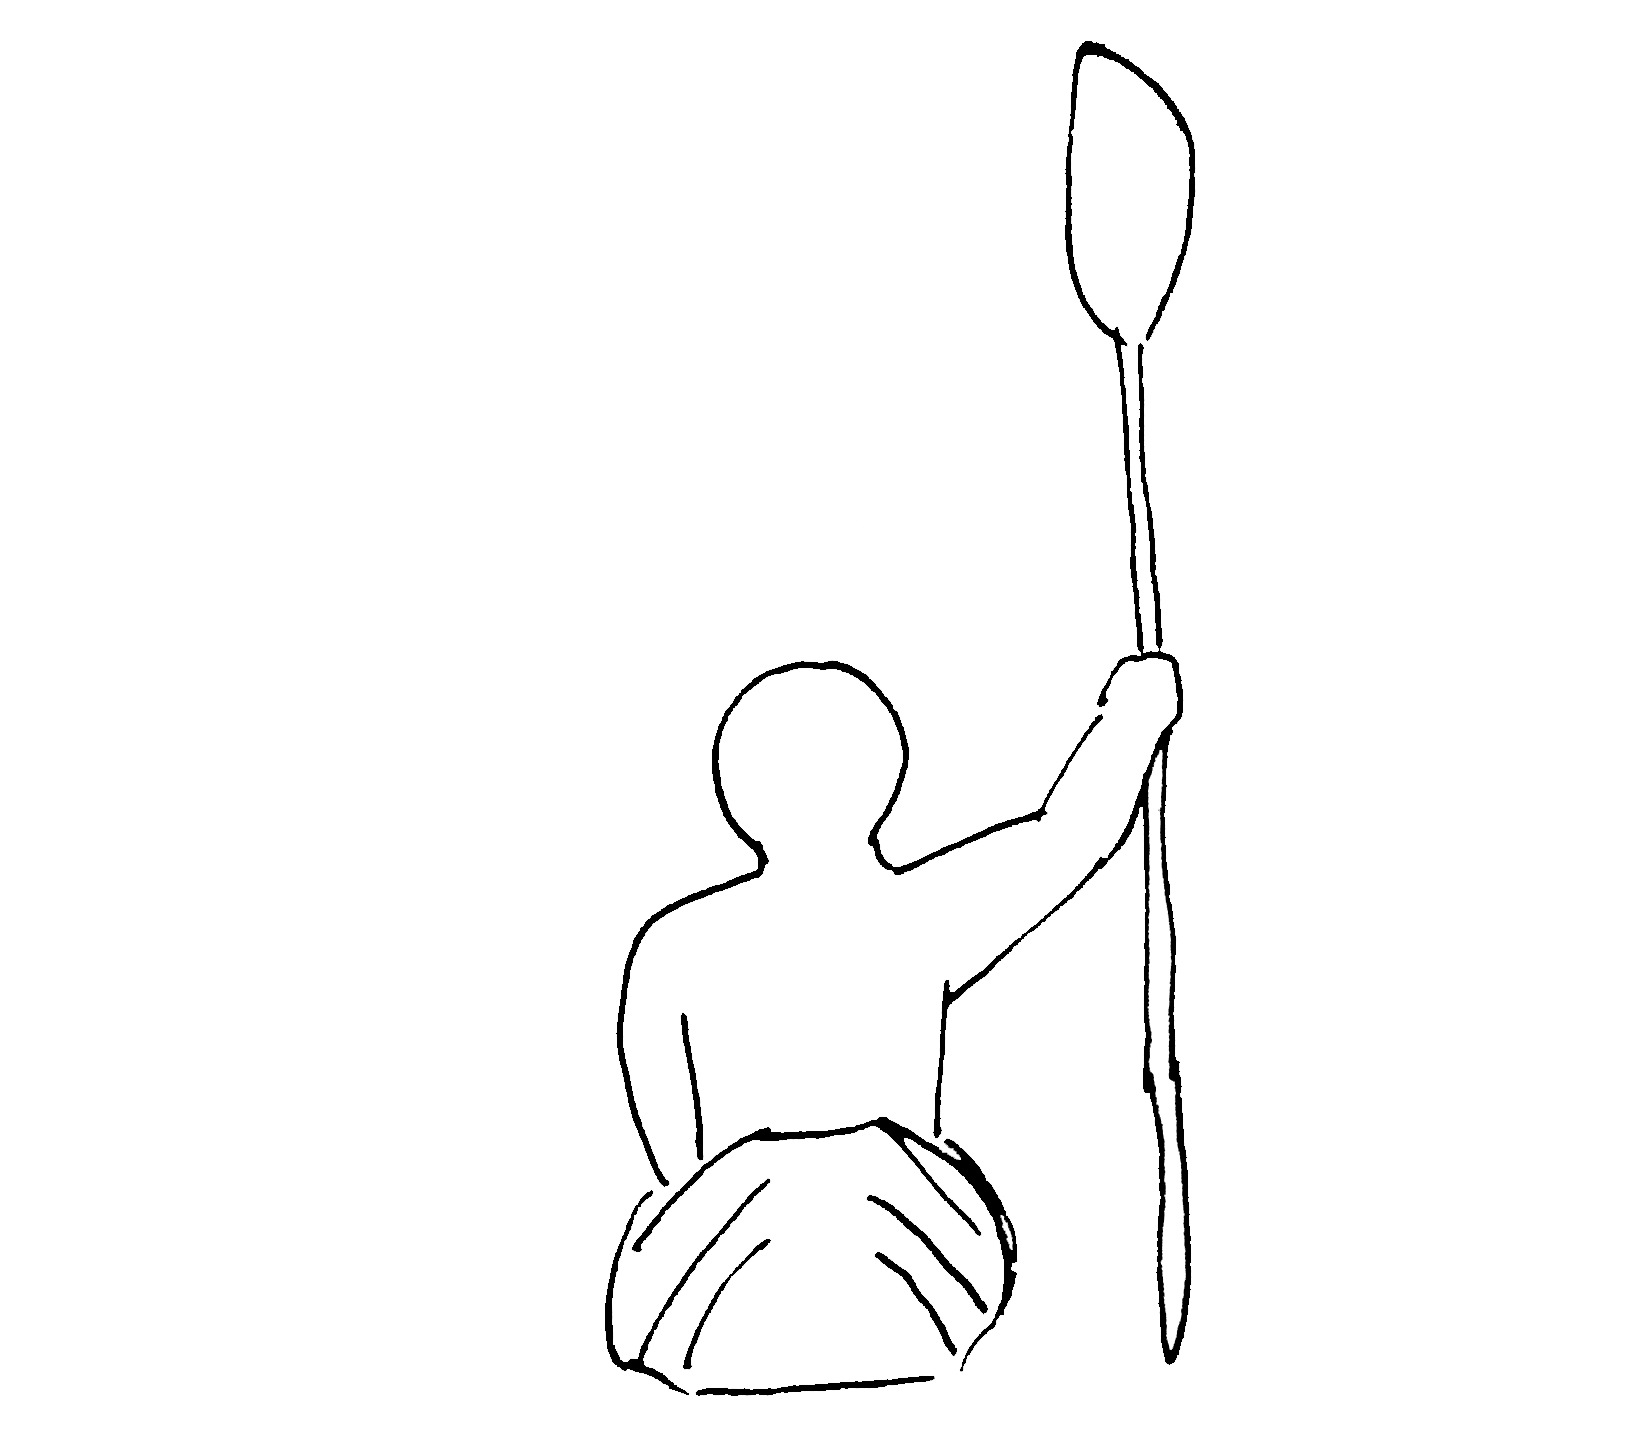
\includegraphics[width=150px]{images/znak_1_plyn.jpg}
    \caption*{Płyń}
  \end{subfigure}
  \hfill
  \begin{subfigure}[t]{0.48\linewidth}
    \centering
    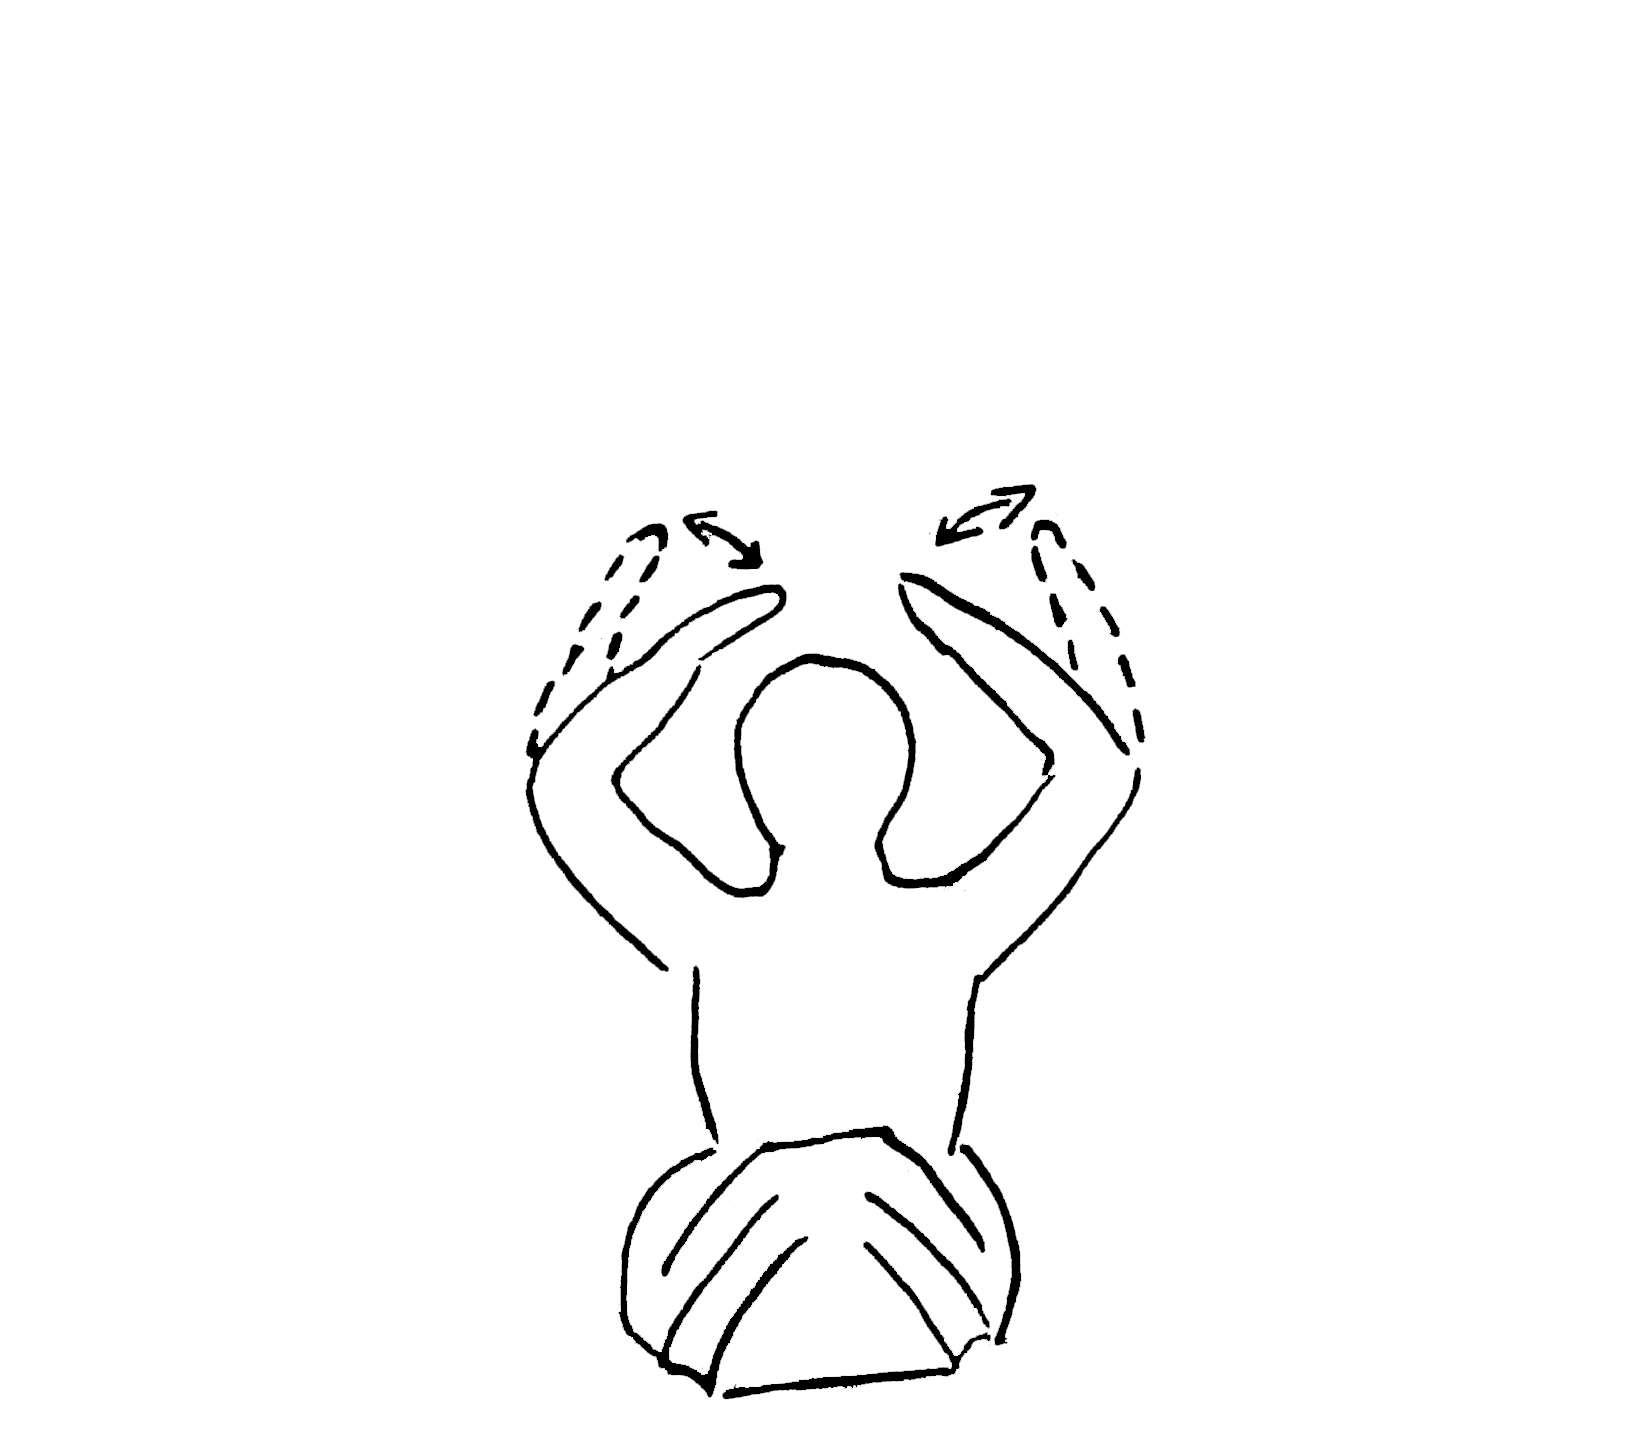
\includegraphics[width=150px]{images/znak_2_do_mnie.jpg}
    \caption*{Do mnie}
  \end{subfigure}
  \begin{subfigure}[t]{0.48\linewidth}
    \centering
    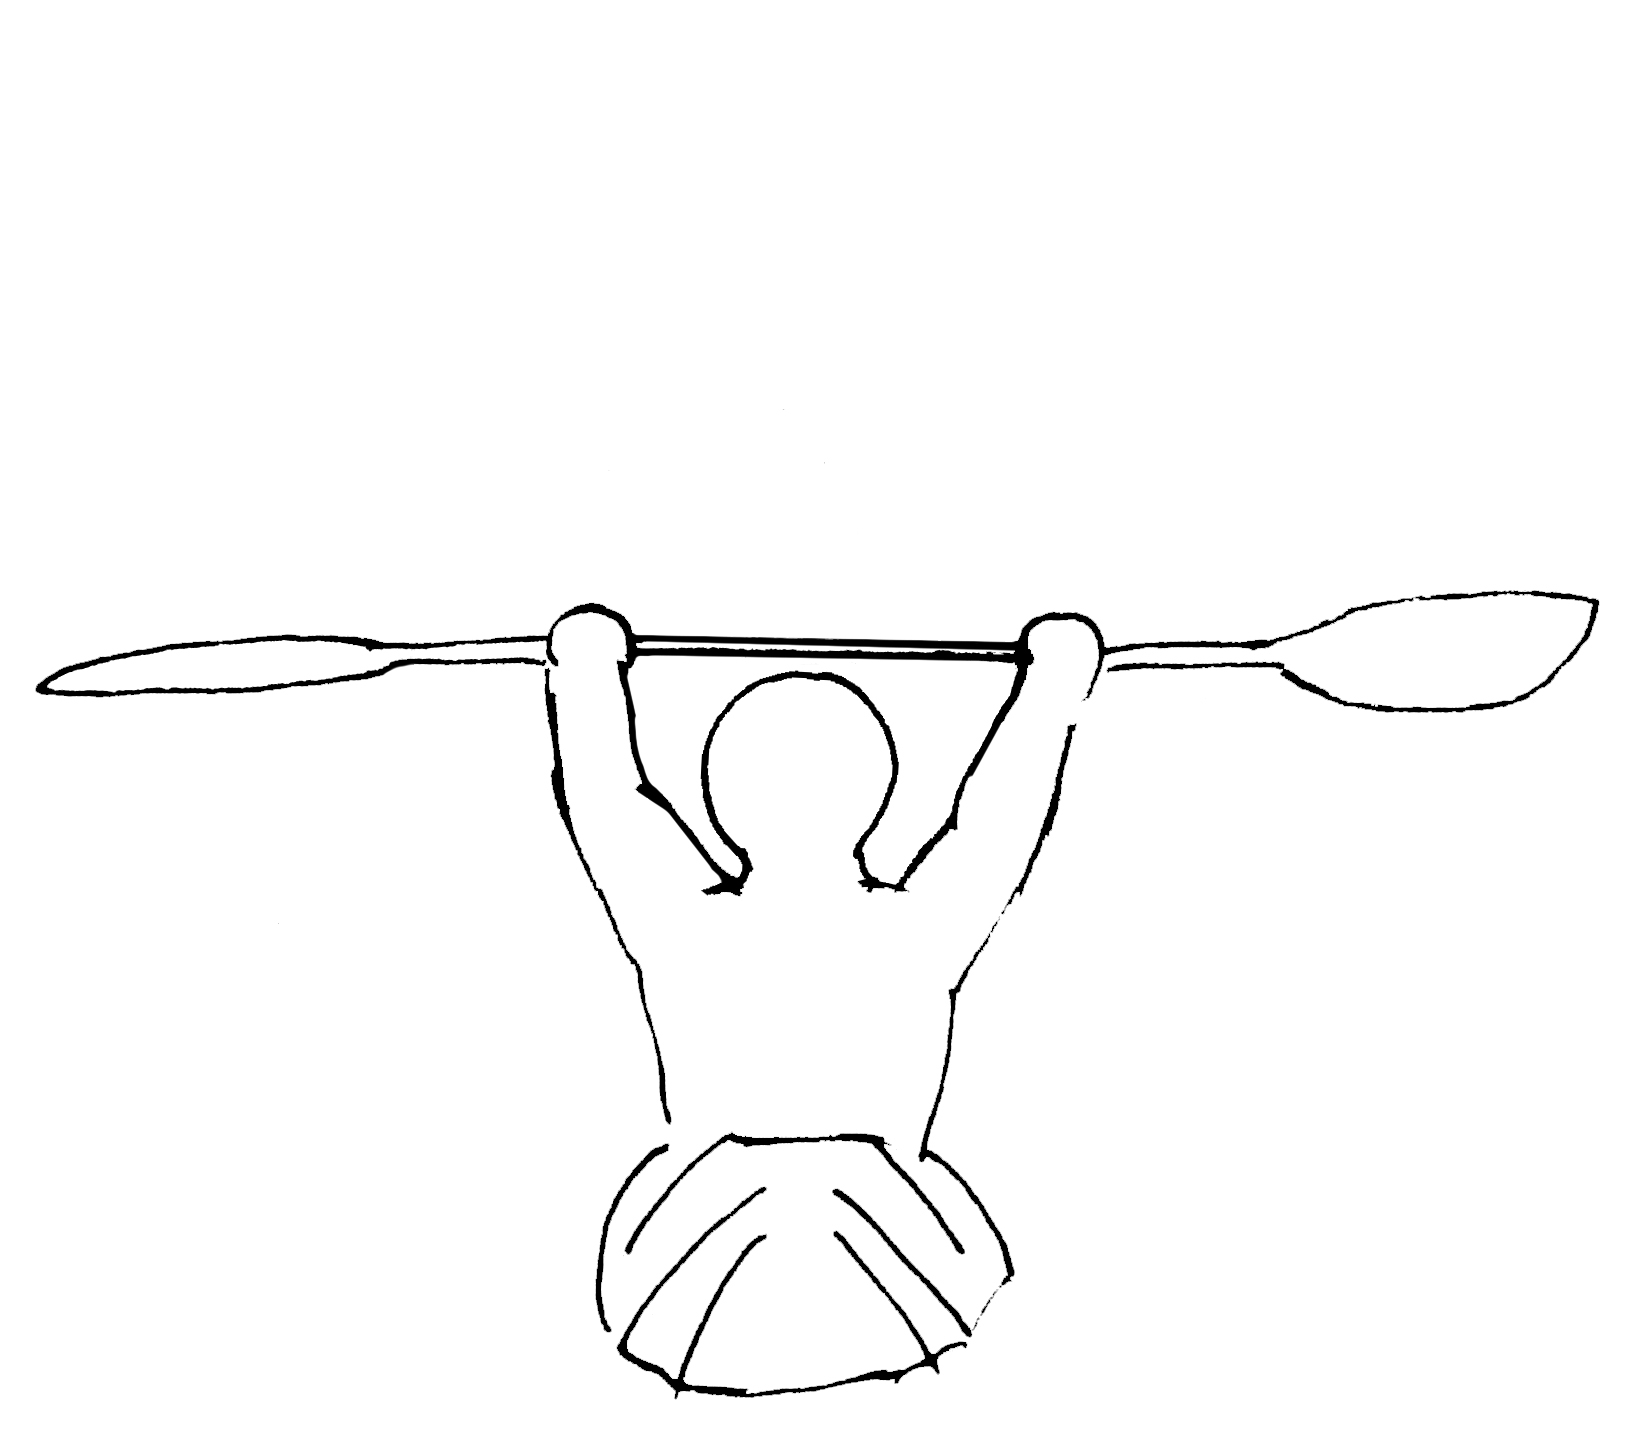
\includegraphics[width=150px]{images/znak_3_stop.jpg}
    \caption*{Stop}
  \end{subfigure}
  \hfill
  \begin{subfigure}[t]{0.48\linewidth}
    \centering
    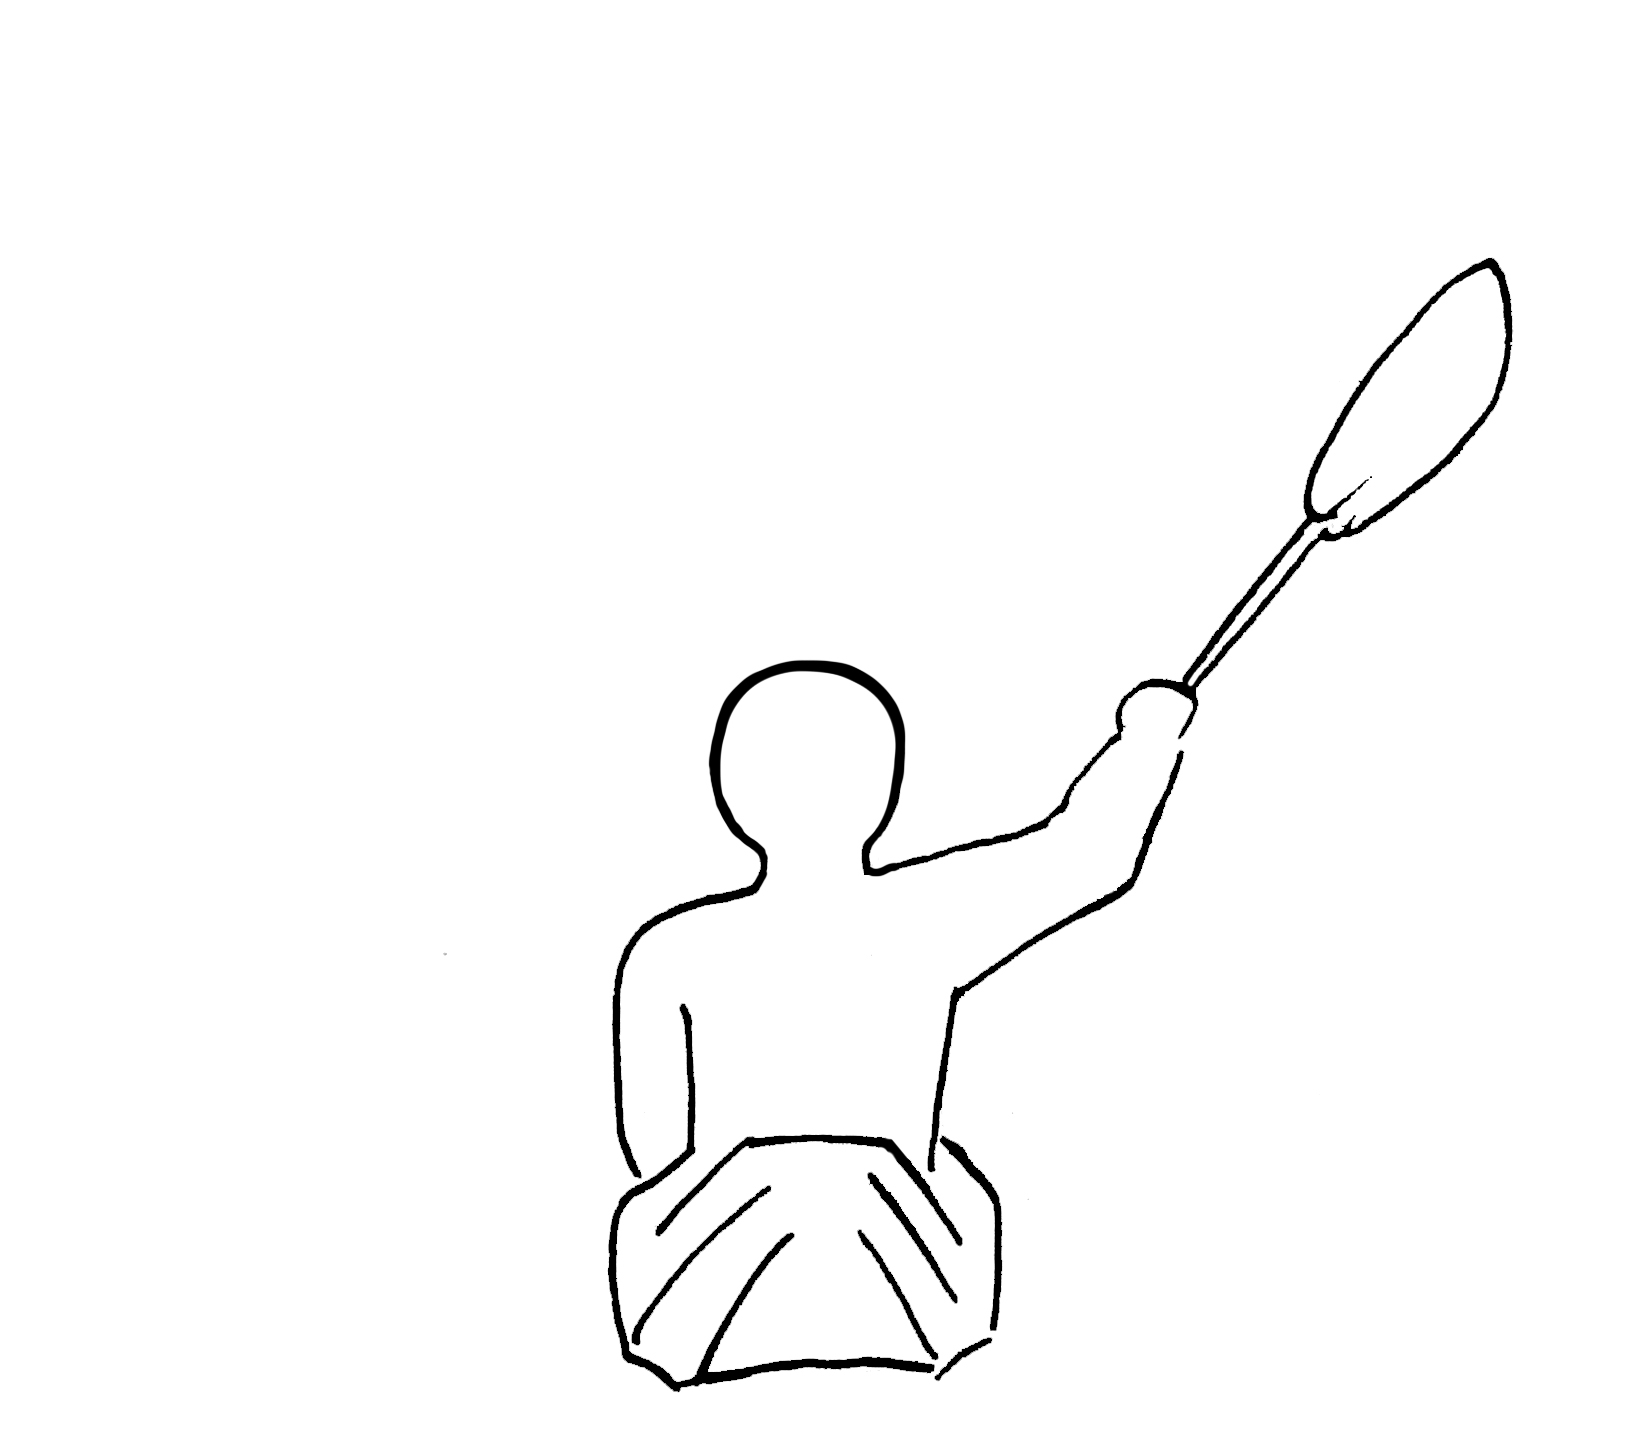
\includegraphics[width=150px]{images/znak_4_plyn_ta_strona.jpg}
    \caption*{Płyń tą stroną}
  \end{subfigure}
  \begin{subfigure}[t]{0.48\linewidth}
    \centering
    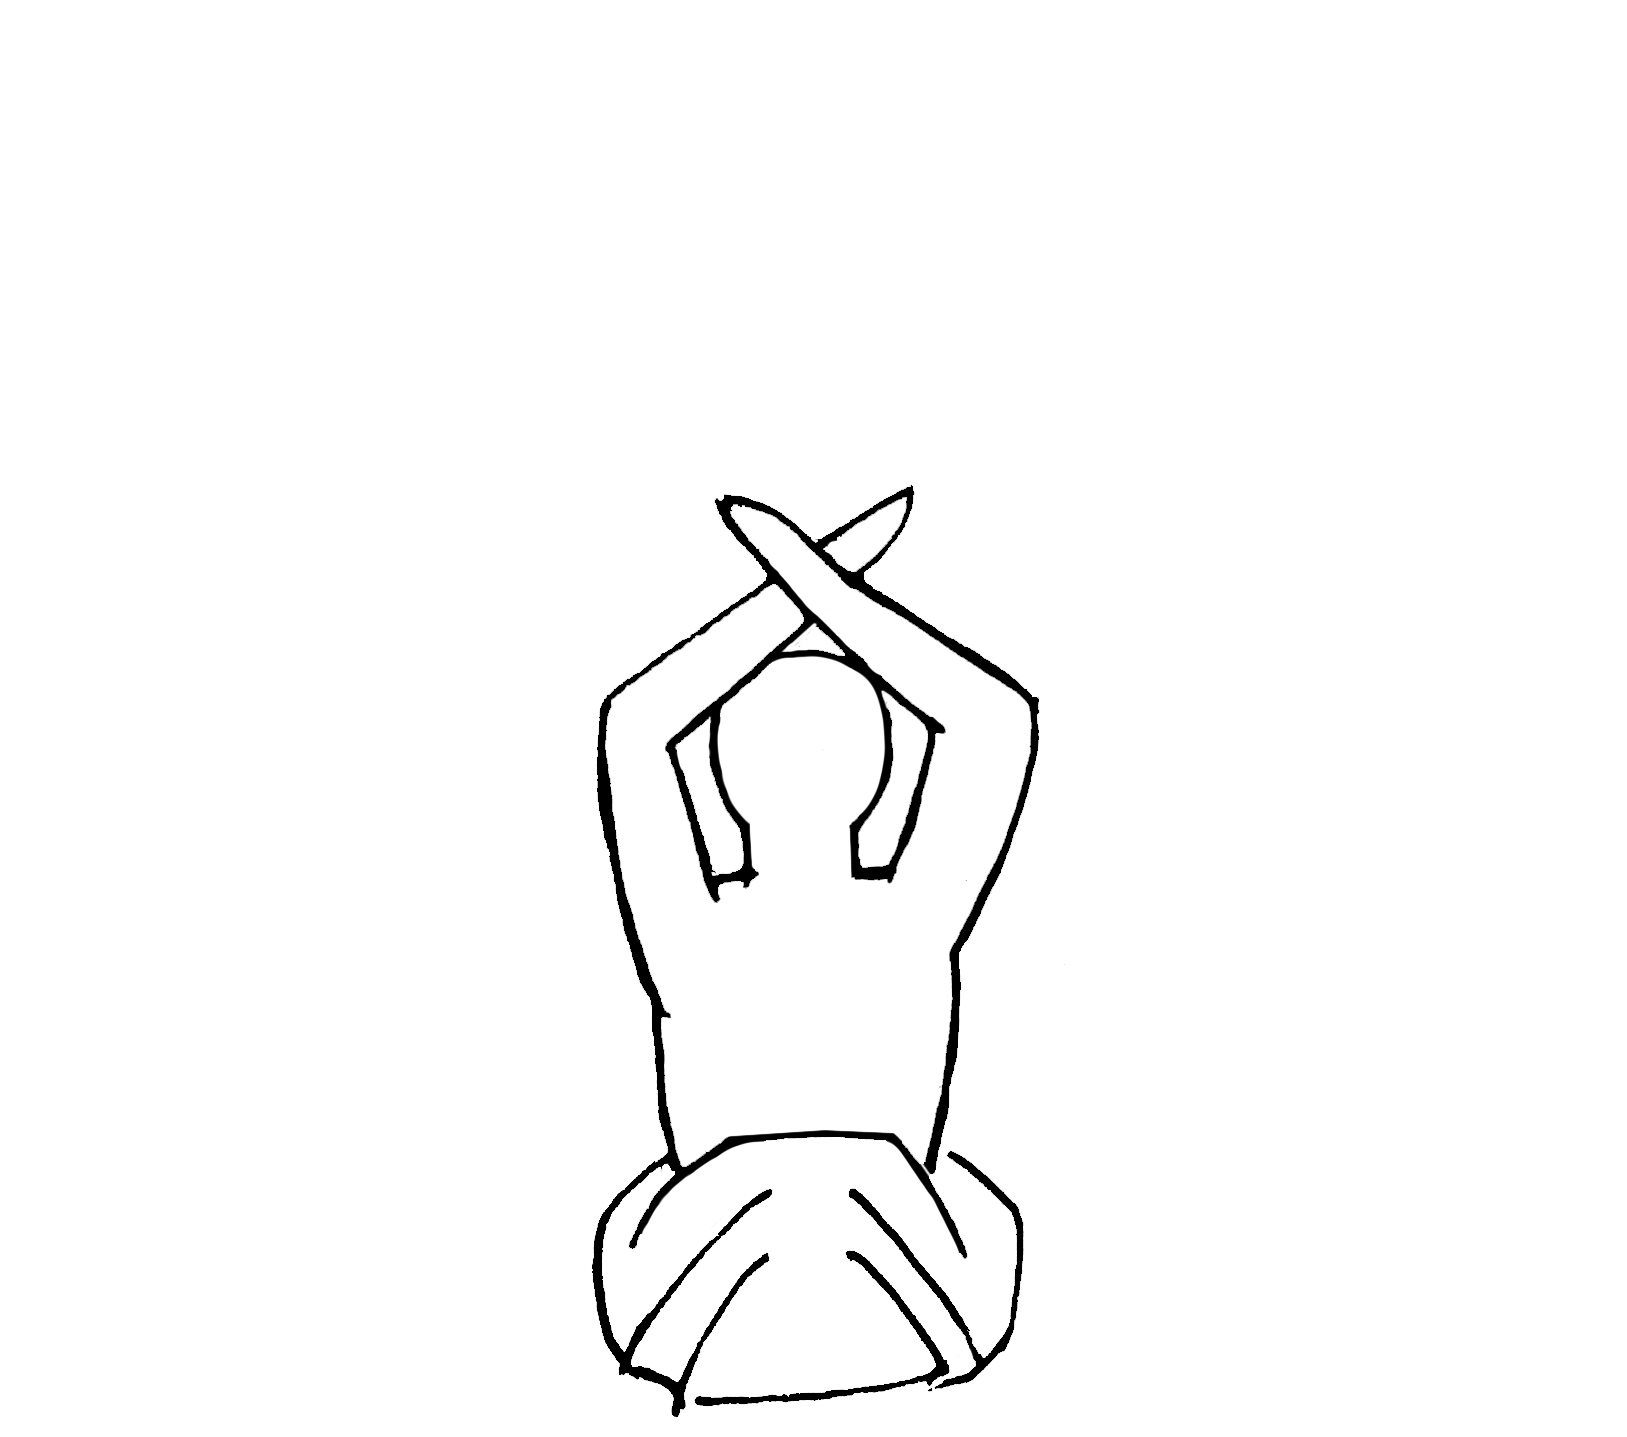
\includegraphics[width=150px]{images/znak_5_koniec.jpg}
    \caption*{Koniec/odcinek niespływalny}
  \end{subfigure}
  \hfill
  \begin{subfigure}[t]{0.48\linewidth}
    \centering
    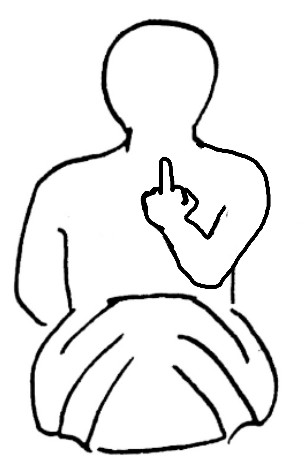
\includegraphics[width=50px]{images/znak_6_srodkiem.jpg}
    \caption*{Płyń środkiem}
  \end{subfigure}
  \begin{subfigure}[t]{0.48\linewidth}
    \centering
    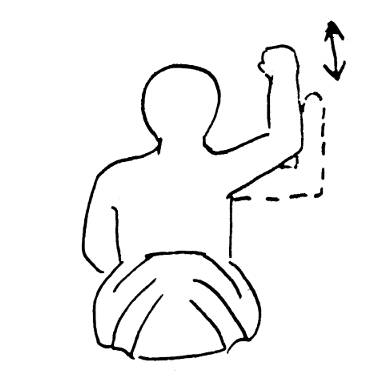
\includegraphics[width=100px]{images/znak_7_przyspiesz.png}
    \caption*{Przyspiesz}
  \end{subfigure}
  \hfill
  \begin{subfigure}[t]{0.48\linewidth}
    \centering
    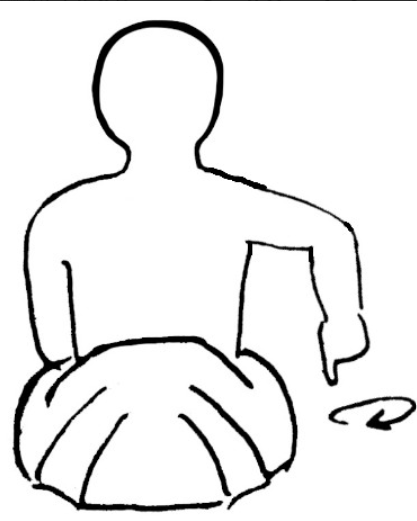
\includegraphics[width=75px]{images/znak_8_cofka.png}
    \caption*{Złap cofkę}
  \end{subfigure}
\end{figure}

\newpage

\begin{figure}[H]
  \ContinuedFloat
  \centering
  \begin{subfigure}[t]{0.48\linewidth}
    \centering
    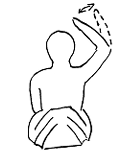
\includegraphics[width=100px]{images/znak_9_ok.png}
    \caption*{Wszystko w porządku}
  \end{subfigure}
  \hfill
  \begin{subfigure}[t]{0.48\linewidth}
    \centering
    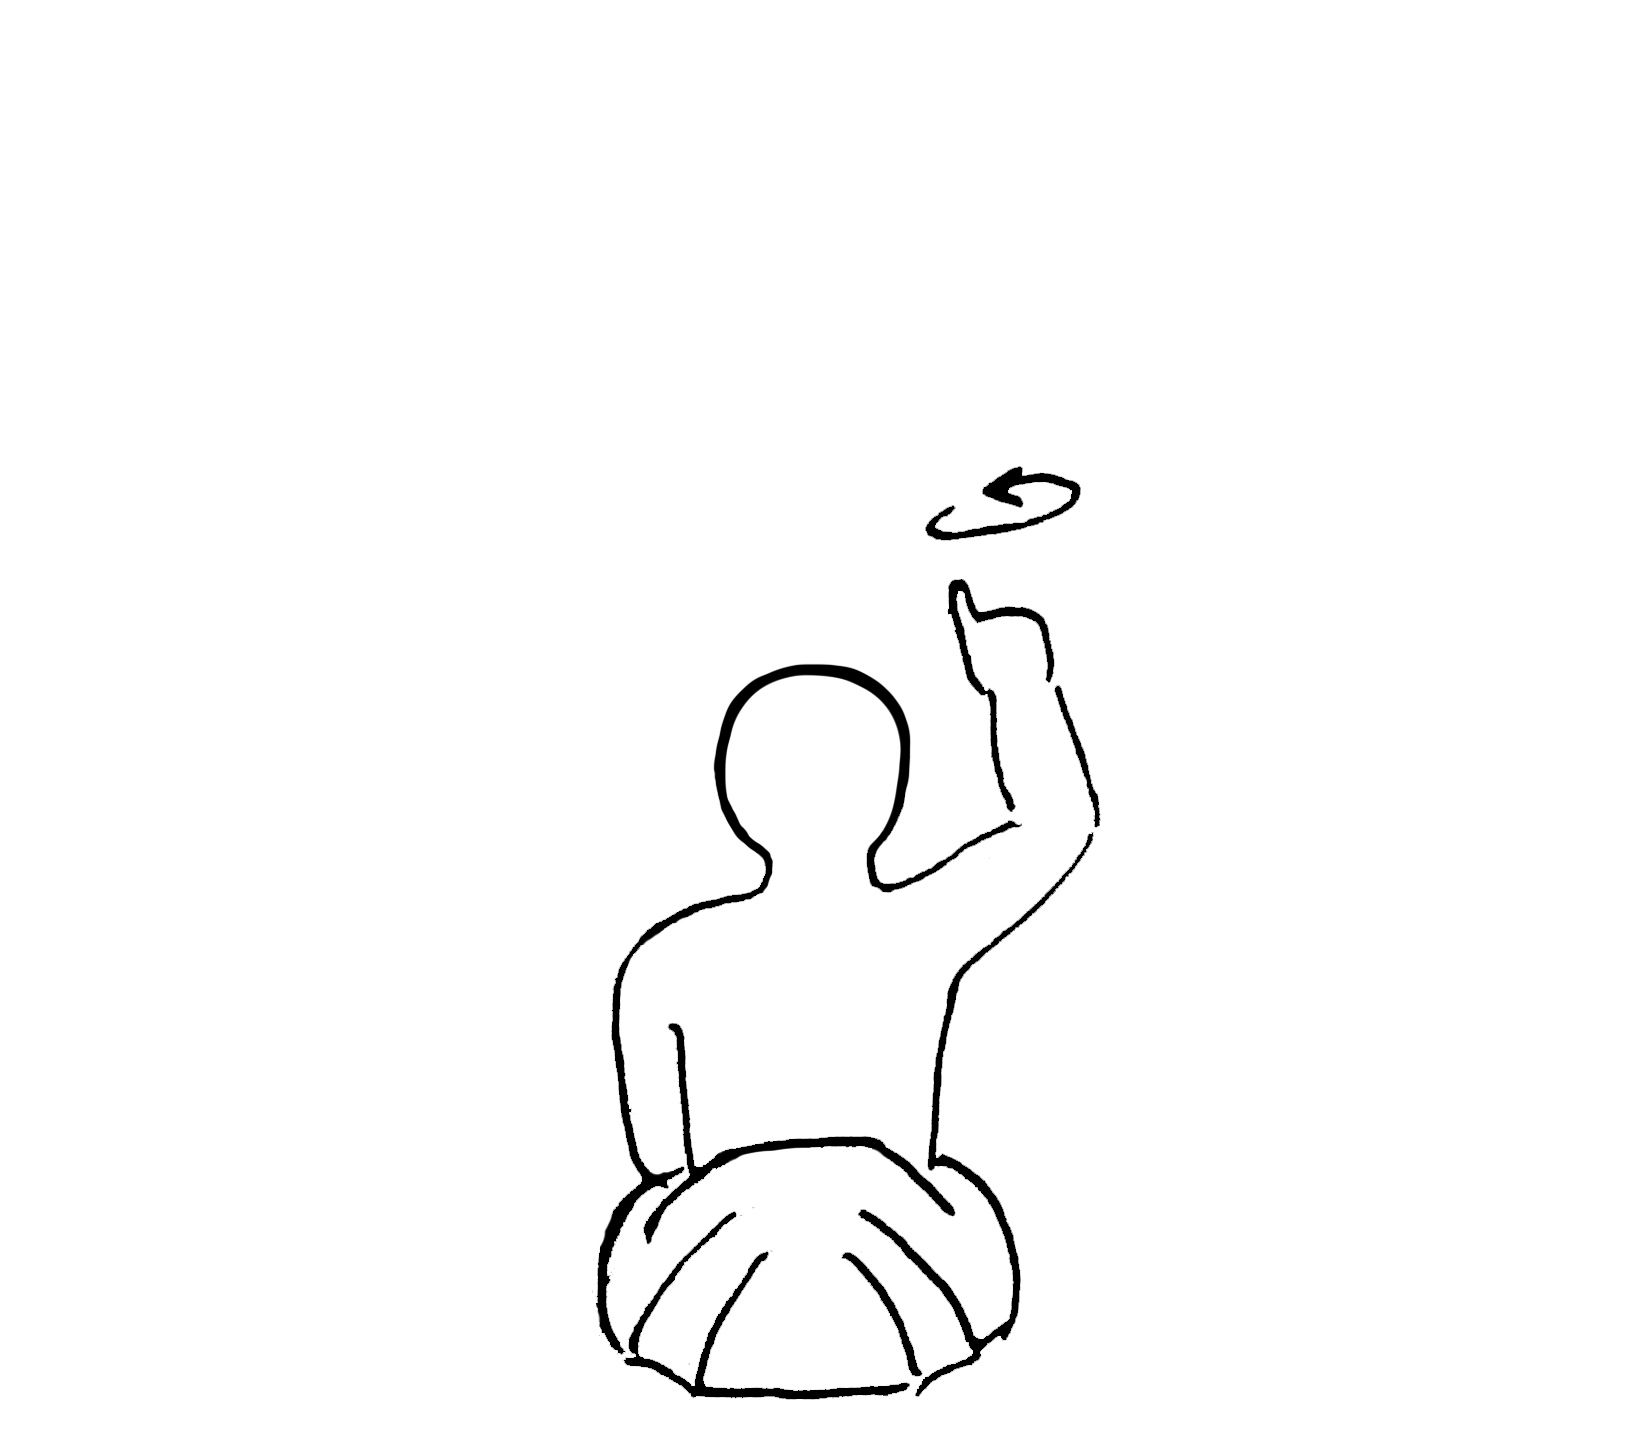
\includegraphics[width=200px]{images/znak_10_kabina.jpg}
    \caption*{Kabina}
  \end{subfigure}
  \begin{subfigure}[t]{0.48\linewidth}
    \centering
    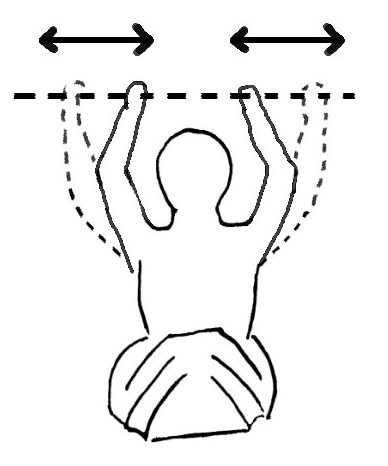
\includegraphics[width=100px]{images/znak_11_wioslo.jpg}
    \caption*{Szukamy wiosła}
  \end{subfigure}
\end{figure}
% ------------------------------------------------------------
\subsection{Komunikacja na wodzie}
% ------------------------------------------------------------

Szum na rzece górskiej nie zawsze pozwala na komunikację werbalną, dlatego przed zejściem na wodę warto ustalić zestaw znaków. Znaki powinny być zawsze przekazane do kolejnej osoby
w szyku i potwierdzone przez każdego członka grupy (jak „głuchy telefon" rękami) — dzięki temu mamy pewność, że dotarły do wszystkich.

Najczęściej używane znaki:

\begin{itemize}[leftmargin=1.5em, itemsep=6pt]
  \item \textbf{Płyń}
  \item \textbf{Stop}
  \item \textbf{Koniec / odcinek niespływalny}
  \item \textbf{Do mnie}
  \item \textbf{Płyń tą stroną}
  \item \textbf{Płyń środkiem}
  \item \textbf{Przyspiesz}
  \item \textbf{Wszystko w porządku}
  \item \textbf{Wiosło}
  \item \textbf{Złap cofkę}
  \item \textbf{Kabina}
\end{itemize}

% ------------------------------------------------------------
\subsection{Filary bezpieczeństwa}
% ------------------------------------------------------------

\subsubsection{Filar 1 — Odpowiednie planowanie}

Dobrze przygotowany spływ pozwala nie tylko uniknąć zagrożeń, ale także zwiększa komfort
uczestników. Proces planowania powinien uwzględniać:

\begin{description}[leftmargin=1.5em, font=\bfseries, style=nextline]

  \item[Dopasowanie poziomu trudności do grupy]
    Należy wziąć pod uwagę wiek, kondycję fizyczną, doświadczenie kajakowe oraz umiejętność
    pływania uczestników.

  \item[Sprzęt dostosowany do umiejętności i trudności spływu]
    Kajaki, wiosła, kamizelki oraz dodatkowe wyposażenie muszą być dostosowane zarówno
    do poziomu zaawansowania uczestników, jak i do charakteru rzeki.

  \item[Zaplanowanie trasy]
    Obejmuje wybór miejsca startu (\emph{put in}) i zakończenia (\emph{take out}), określenie
    długości odcinka i czasu potrzebnego na jego pokonanie. Należy uwzględnić możliwość
    przerw, miejsc biwakowych oraz punktów ewakuacyjnych.

  \item[Warunki atmosferyczne i hydrologiczne]
    Przed wyprawą sprawdź prognozę pogody (opady, temperatura, burze) oraz warunki
    hydrologiczne (poziom wody, prędkość nurtu). Zbyt wysoki lub gwałtownie zmieniający się
    stan rzeki może znacząco zwiększyć stopień trudności spływu.

  \item[Plan awaryjny — plan B, C, a nawet D i E]
    Każdy spływ powinien mieć przygotowany plan awaryjny: skrócenie trasy, zmianę miejsca
    zakończenia lub przerwanie spływu. Elastyczność i gotowość do zmiany pierwotnych założeń
    są niezbędne dla bezpieczeństwa całej grupy.

\end{description}

% ............................................................
\subsubsection{Filar 2 — Wzajemna asekuracja}

\begin{warnbox}
  Kajakarstwo to \textbf{nie} jest sport indywidualny!
\end{warnbox}

Zasady do zapamiętania:

\begin{itemize}[leftmargin=1.5em, itemsep=2pt]
  \item Pomagamy sobie nawzajem.
  \item Trzymamy się grupy.
  \item Słuchamy kierownika.
  \item \textbf{Klepiemy o dzioba!!!}
  \item Obstawiamy miejsca.
  \item Łowimy kabiny.
  \item Podajemy dzióbki.
  \item Ogarniamy się po kabinie.
\end{itemize}

\paragraph{Dzióbek}

Manewr ratowniczy polegający na wykorzystaniu dziobu kajaka partnera w celu wynurzenia się przewróconego kajakarza. Jest to jedna z podstawowych technik asekuracji zespołowej,
szczególnie przydatna dla osób, które nie opanowały jeszcze eskimoski.

Manewr rozpoczyna się w momencie wywrotki. Zamiast podejmować próbę kabinowania się, kajakarz wyciąga dłonie po obu stronach wywróconego kajaka i mocno uderza w burty —
alarmuje tym kajakarzy w okolicy. Partner podpływa do burty prostopadle. Ratowany chwyta dziób kajaka partnera, który stanowi stabilny punkt podparcia umożliwiający wynurzenie się.

\begin{figure}[H]
    \centering
    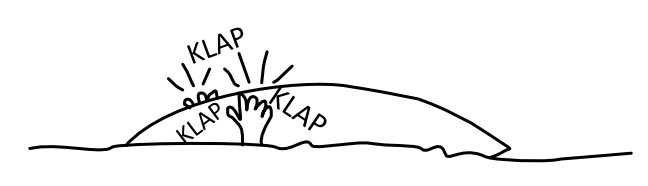
\includegraphics[width=400px]{images/dzióbek.jpg}
    \caption{Wizualizacja zachowania kajakarza wołającego o dzióbek}
\end{figure}

\paragraph{Kabina}

Kabinowanie to manewr pozwalający na szybką i bezpieczną ewakuację z kajaka po wywrotce.
Celem jest wydostanie się z kokpitu bez paniki.

\begin{enumerate}[leftmargin=1.5em, itemsep=2pt]
  \item Zachowaj spokój. Pochyl się do przodu — twarz jak najbliżej fartucha
    (\emph{zasada „kryj ryj"}).
  \item Chwyć ucho fartucha i mocno pociągnij do góry i do siebie.
  \item Wykonaj kontrolowane podciągnięcie nóg w kierunku kokpitu.
  \item Przesuń biodra i tułów w stronę otwarcia kokpitu, wykonując coś w rodzaju
    przewrotu w przód ku powierzchni wody.
\end{enumerate}

\textbf{Co po kabinie?}

Jeśli to możliwe, staraj się utrzymać wiosło — może być pomocne w płynięciu wpław.
Po wynurzeniu bezwzględnie staraj się znaleźć na brzegu lub innym bezpiecznym miejscu
poza nurtem. Jeśli jesteś w bardzo silnym nurcie, przyjmij \textbf{pozycję bezpieczną}:
twarz skierowana w dół rzeki, stopy uniesione i skierowane w dół rzeki.

\begin{figure}[H]
    \centering
    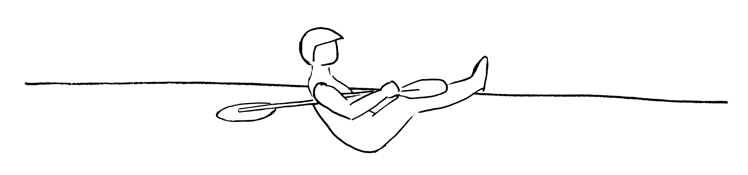
\includegraphics[width=400px]{images/pozycja_bezpieczna.png}
    \caption{Wizualizacja płynięcia w pozycji bezpiecznej}
\end{figure}

\begin{warnbox}
  W nurcie bezwzględnie zakazane jest chodzenie po dnie — istnieje ryzyko zaklinowania
  stopy i utknięcia głową pod wodą.
\end{warnbox}

Pozostali kajakarze często podejmują pływaka na dziób lub rufę:

\begin{itemize}[leftmargin=1.5em, itemsep=3pt]
  \item \textbf{Podjęcie na dziób (Koala)} — chwytamy dziób ratującego; głowa z boku
    dziobu, nigdy przed nim. Jeśli mamy siłę, pomagamy ratującemu przebierając nogami.
  \item \textbf{Podjęcie na rufę} — chwytamy uchwyt na rufie jedno- lub oburącz,
    przyjmując pozycję „supermana".
\end{itemize}

\begin{figure}[H]
    \centering
    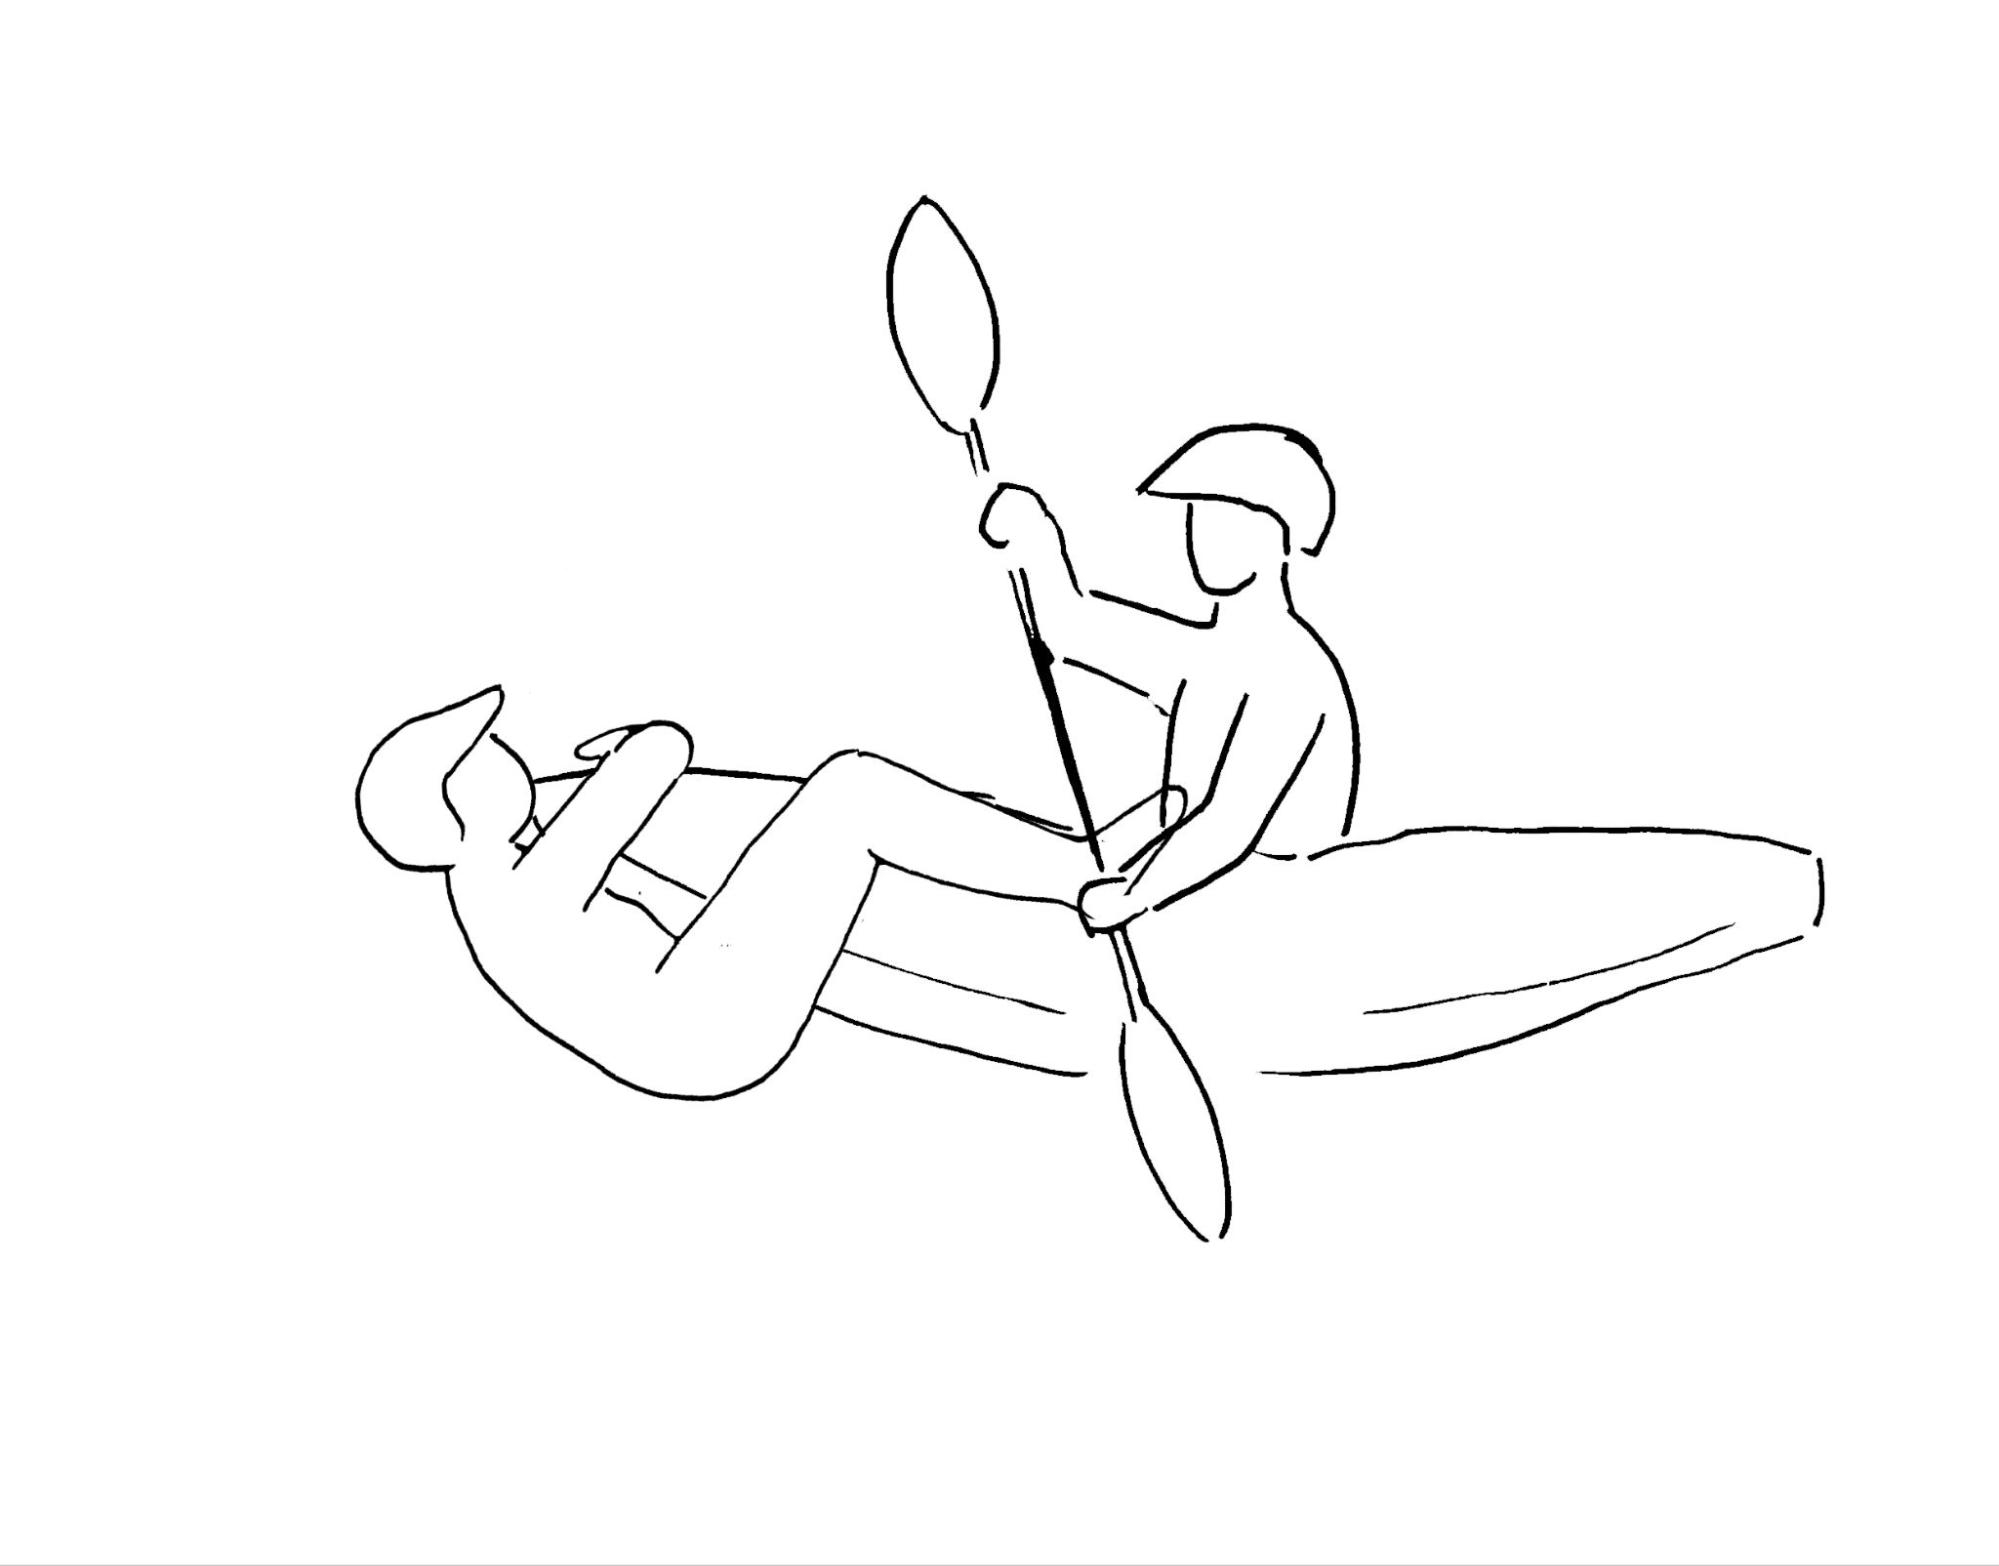
\includegraphics[width=300px]{images/koala.jpg}
    \caption{Wizualizacja manewru holowania na dziobie - koala}
\end{figure}

\begin{tipbox}
  Bezwzględnie stosujemy się do poleceń ratującego. Nigdy nie łapiemy za \textbf{burtę} ratującego — możemy w ten sposób wywrócić naszego ratownika.
\end{tipbox}

\paragraph{Eskimoska}

Eskimoska (rolka) to manewr pozwalający kajakarzowi odwrócić się do pozycji pionowej
po wywrotce bez wychodzenia z kajaka. Opiera się na połączeniu pracy bioder, tułowia
i wiosła.

Ruch powinien być zapoczątkowany z biodra — wykorzystując opór wody na piórze wiosła,
wynurzamy tułów, kontrolując aby \textbf{głowa wynurzyła się na samym końcu}. Kluczowe jest
właściwe wstępne ustawienie wiosła względem kajaka.

\paragraph{Ręka boga}

Manewr ratowniczy używany gdy kajakarz jest przewrócony do góry dnem i nie może sam powrócić
do pionu. Kajakarz asekurujący podpływa obok przewróconego kajaka, sięga ręką i łapie za
rant kokpitu od strony dalszej od siebie. Następnie, naciskając jedną ręką na bliższy bok
i pociągając drugą za dalszy rant, obraca kajak do pozycji pionowej.

Ratowany zawsze utrzymuje pozycję pochyloną do przodu z twarzą jak najbliżej fartucha —
pomaga to ratującemu w wykonaniu manewru.

\paragraph{Asekuracja z brzegu}

Polega na zabezpieczeniu kajakarza znajdującego się w nurcie lub po wywrotce. Osoba
asekurująca stoi mocno w rozkroku lub za kotwicą (np. stabilnym kamieniem).

\textbf{Rzucanie rzutką} wymaga precyzji i przewidzenia nurtu. Przy rzucaniu:

\begin{itemize}[leftmargin=1.5em, itemsep=2pt]
  \item Stój stabilnie na brzegu, \textbf{nigdy} w nurcie.
  \item Nawiąż kontakt wzrokowy z ratowanym i krzyknij \textbf{„RZUTKA!"}
    przed każdym rzutem.
  \item Celuj \emph{przed} kajakarzem — nie w niego bezpośrednio.
  \item Wypuszczaj rzutkę nad wodą, aby lina nie zahaczała o przeszkody.
\end{itemize}

Ratowany po chwyceniu rzutki powinien obrócić się na plecy i skośnie przełożyć linę przed klatką piersiową, po tej samej stronie głowy co ratownik, aby uniemożliwić jej zaplątanie się wokół szyi.

\begin{figure}[H]
    \centering
    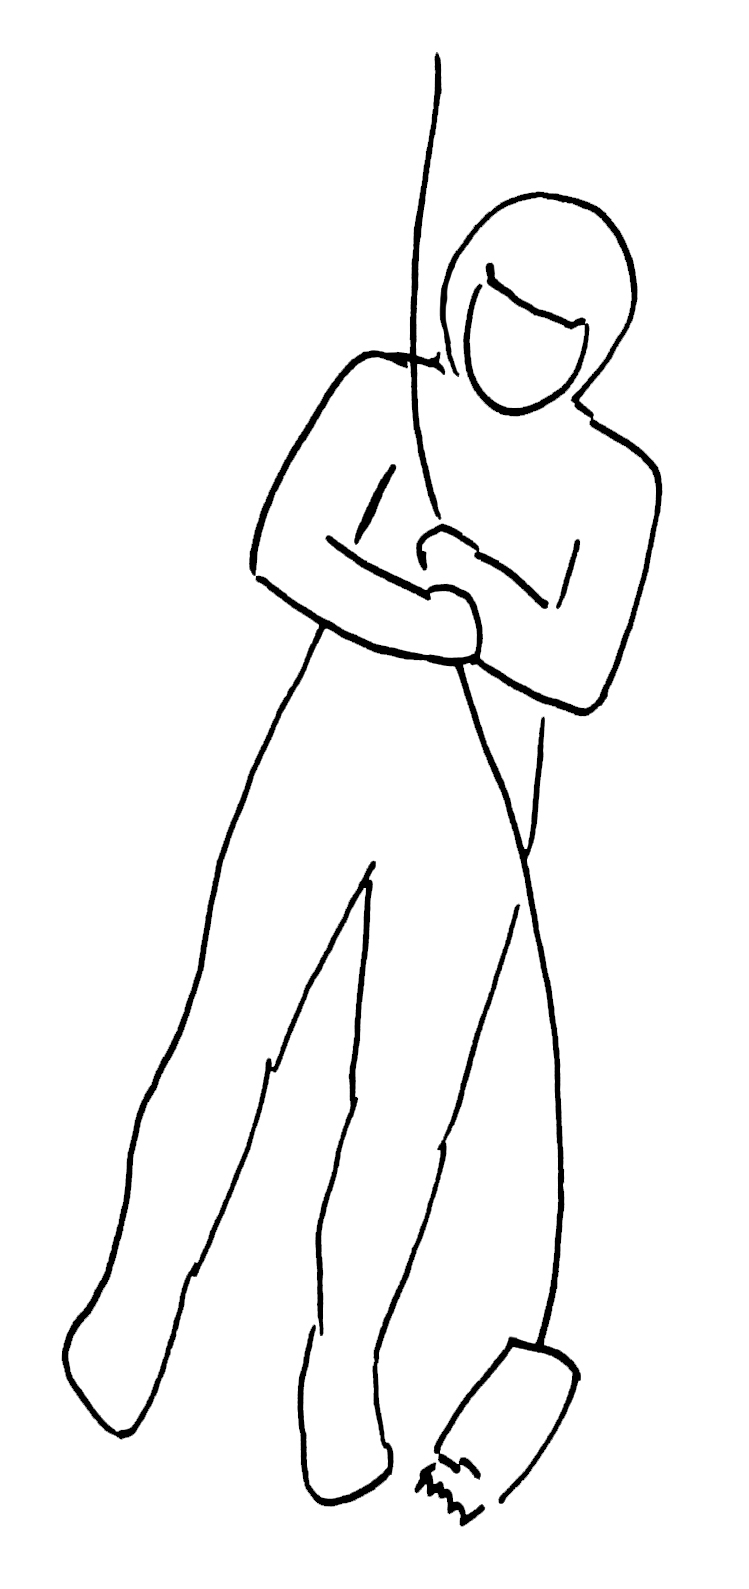
\includegraphics[width=100px]{images/rzutka.jpg}
    \caption{Ułozenie ratowanego po złapaniu rzutki}
\end{figure}

% ............................................................
\subsubsection{Filar 3 — Jednoosobowe kierownictwo}

Jednoosobowe kierownictwo polega na powierzeniu odpowiedzialności za organizację,
bezpieczeństwo i podejmowanie kluczowych decyzji jednej, wyznaczonej osobie —
\textbf{komandorowi spływu}. Na wodzie często dochodzi do sytuacji wymagających
natychmiastowej reakcji; brak jednoznacznego lidera może prowadzić do chaosu.

\begin{warnbox}
  Nigdy nie podważamy decyzji osoby, która rozpoczęła kierownictwo akcją ratunkową.
\end{warnbox}

Cechy komandora spływu:

\begin{description}[leftmargin=1.5em, font=\bfseries, style=nextline]

  \item[Znajomość odcinka rzeki]
    Wiedza o charakterze trasy, miejscach niebezpiecznych, przeszkodach wodnych
    i możliwościach ewakuacji pozwala na odpowiednie przygotowanie i szybkie reagowanie.

  \item[Doświadczenie kajakowe]
    Umożliwia trafną ocenę warunków hydrologicznych i atmosferycznych oraz przewidywanie
    potencjalnych zagrożeń.

  \item[Zdecydowanie]
    Komandor musi potrafić jasno wydawać polecenia i egzekwować ich wykonanie, nawet gdy
    są niepopularne (np. przerwanie spływu lub zmiana trasy).

  \item[Umiejętność działania pod presją]
    Sytuacje awaryjne wiążą się z presją czasu. Komandor powinien zachować spokój, logicznie
    analizować sytuację i podejmować racjonalne decyzje minimalizujące ryzyko dla grupy.

\end{description}

% ------------------------------------------------------------
\subsection{Szyk płynięcia}
% ------------------------------------------------------------

\begin{description}[leftmargin=1.5em, font=\bfseries]
  \item[Zielona Latarnia]
    Pierwsza płynąca osoba (otwierający). Płynie pierwszy, wyznacza linię płynięcia —
    nie wyprzedza się jej.
  \item[Czerwona Latarnia]
    Ostatnia płynąca osoba. Nikt nie pozostaje za nią.
\end{description}

% ------------------------------------------------------------
\subsection{Apteczka}
% ------------------------------------------------------------

\begin{longtable}{>{\bfseries}p{5.5cm} >{\centering}p{1.8cm} p{6.5cm}}
  \toprule
  \textbf{Element} & \textbf{Ilość} & \textbf{Zastosowanie} \\
  \midrule
  \endfirsthead
  \toprule
  \textbf{Element} & \textbf{Ilość} & \textbf{Zastosowanie} \\
  \midrule
  \endhead
  \bottomrule
  \endfoot

  Rękawiczki                       & 3--4 pary  & Ochrona ratownika \\
  Gaza jałowa                      & 5--8 szt.  & Opatrywanie ran \\
  Bandaż elastyczny                & 2 szt.     & Skręcenia, stabilizacja \\
  Bandaż zwykły                    & 2 szt.     & Mocowanie opatrunków \\
  Bandaż elastyczny siatkowy       & 1 szt.     & Mocowanie opatrunków \\
  Plastry z opatrunkiem            & zestaw     & Drobne rany \\
  Plastry ściągające (stripy)      & 1 zestaw   & Zamknięcie ran ciętych \\
  Plaster w rolce (mocny)          & 1 szt.     & Mocowanie, wzmacnianie \\
  Taśma izolacyjna (PVC)*          & 1 rolka    & Usztywnienia, naprawy, opatrunki awaryjne \\
  Chusta trójkątna                 & 1 szt.     & Unieruchomienie kończyn \\
  Koc termiczny (NRC)              & 1--2 szt.  & Ochrona przed hipotermią \\
  Środek do dezynfekcji            & 1 szt.     & Oczyszczanie ran \\
  Opaska uciskowa / staza          & 1 szt.     & Masowe krwotoki \\
  Nożyczki ratownicze              & 1 szt.     & Cięcie ubrań, bandaży \\
  Maska do RKO                     & 1 szt.     & Bezpieczna resuscytacja \\
  Pęseta                           & 1 szt.     & Drzazgi, kleszcze \\
  Folia / etui wodoszczelne        & 1 szt.     & Ochrona apteczki \\
  Instrukcja pierwszej pomocy      & 1 szt.     & Wsparcie w stresie \\
  Lista wyposażenia apteczki       & 1 szt.     & Rewizja i uzupełnienie \\
\end{longtable}